\documentclass[ignorenonframetext,]{beamer}
\setbeamertemplate{caption}[numbered]
\setbeamertemplate{caption label separator}{: }
\setbeamercolor{caption name}{fg=normal text.fg}
\beamertemplatenavigationsymbolsempty
\usepackage{lmodern}
\usepackage{amssymb,amsmath}
\usepackage{ifxetex,ifluatex}
\usepackage{fixltx2e} % provides \textsubscript
\ifnum 0\ifxetex 1\fi\ifluatex 1\fi=0 % if pdftex
  \usepackage[T1]{fontenc}
  \usepackage[utf8]{inputenc}
\else % if luatex or xelatex
  \ifxetex
    \usepackage{mathspec}
  \else
    \usepackage{fontspec}
  \fi
  \defaultfontfeatures{Ligatures=TeX,Scale=MatchLowercase}
\fi
\usetheme[]{Szeged}
\usefonttheme{professionalfonts}
% use upquote if available, for straight quotes in verbatim environments
\IfFileExists{upquote.sty}{\usepackage{upquote}}{}
% use microtype if available
\IfFileExists{microtype.sty}{%
\usepackage{microtype}
\UseMicrotypeSet[protrusion]{basicmath} % disable protrusion for tt fonts
}{}
\newif\ifbibliography
\usepackage{natbib}
\bibliographystyle{plainnat}
\hypersetup{
            pdftitle={MOEA/D},
            pdfborder={0 0 0},
            breaklinks=true}
\urlstyle{same}  % don't use monospace font for urls
\usepackage{graphicx,grffile}
\makeatletter
\def\maxwidth{\ifdim\Gin@nat@width>\linewidth\linewidth\else\Gin@nat@width\fi}
\def\maxheight{\ifdim\Gin@nat@height>\textheight0.8\textheight\else\Gin@nat@height\fi}
\makeatother
% Scale images if necessary, so that they will not overflow the page
% margins by default, and it is still possible to overwrite the defaults
% using explicit options in \includegraphics[width, height, ...]{}
\setkeys{Gin}{width=\maxwidth,height=\maxheight,keepaspectratio}

% Prevent slide breaks in the middle of a paragraph:
\widowpenalties 1 10000
\raggedbottom

\AtBeginPart{
  \let\insertpartnumber\relax
  \let\partname\relax
  \frame{\partpage}
}
\AtBeginSection{
  \ifbibliography
  \else
    \let\insertsectionnumber\relax
    \let\sectionname\relax
    \frame{\sectionpage}
  \fi
}
\AtBeginSubsection{
  \let\insertsubsectionnumber\relax
  \let\subsectionname\relax
  \frame{\subsectionpage}
}

\setlength{\parindent}{0pt}
\setlength{\parskip}{6pt plus 2pt minus 1pt}
\setlength{\emergencystretch}{3em}  % prevent overfull lines
\providecommand{\tightlist}{%
  \setlength{\itemsep}{0pt}\setlength{\parskip}{0pt}}
\setcounter{secnumdepth}{0}


\setbeamertemplate{navigation symbols}{}
\setbeamertemplate{footline}[page number]
\institute{System and Information Engineering}
%\titlegraphic{\includegraphics[width=0.3\paperwidth]{\string~/Dropbox/teaching/clemson-academic.png}}
\setbeamertemplate{title page}[empty]


\AtBeginPart{}
\AtBeginSection{}
\AtBeginSubsection{}
\AtBeginSubsubsection{}
\setlength{\emergencystretch}{0em}
\setlength{\parskip}{0pt}

\title{MOEA/D}
\subtitle{MOEA/D - Restart Strategy}
\author{Yuri Lavinas\\
Master Student - University of Tsukuba}
\date{06/27/2018}

\begin{document}
\frame{\titlepage}

\section{MOP}\label{mop}

\subsection{Multi-objective Problems}\label{multi-objective-problems}

\begin{frame}{What is MOP?}

Multiobjective Optimization Problem have \(m\) multiple objective
functions that must be optimized simultaneously.

Maximize\(^1\) \(F(x) = (f_1(x), f_2(x), ..., f_m(x))\),

subject to \(x\) in \(\Omega\).

\begin{itemize}
\tightlist
\item
  \(F(x)\) objective functions;
\item
  \(f_i\) is the i-th objective to be maximized;
\item
  \(x\) is the decision vector;
\item
  \(\Omega\) is the decision space.
\end{itemize}

\footnotesize \(^1\) All definitions are for maximization. Following
inequalities should be reversed if the goal is to minimize.

\end{frame}

\begin{frame}{Why is MOP interesting?}

\begin{enumerate}
\def\labelenumi{\arabic{enumi}.}
\tightlist
\item
  Many real-world scientific and engineering are MOP.

  \begin{itemize}
  \tightlist
  \item
    Water quality control, Groundwater pollution re-mediation, Design of
    marine vehicles, \ldots{} \citet{coello2007evolutionary}.
  \item
    Petrol extraction.
  \end{itemize}
\item
  Hard problems: to balance the interests of the multi-objective as a
  whole is hard.
\end{enumerate}

\end{frame}

\subsection{Pareto Set}\label{pareto-set}

\begin{frame}{What is Pareto Set?}

Objectives may be conflicting - The goal is to find good trade-off.

\begin{itemize}
\tightlist
\item
  Set of solutions.
\end{itemize}

Set of \emph{optimum solutions} - Pareto set.

\begin{itemize}
\tightlist
\item
  Non-dominated solutions: no single solution provides a better
  trade-off in all objectives.
\end{itemize}

\end{frame}

\begin{frame}{What is Pareto Set?}

\centering
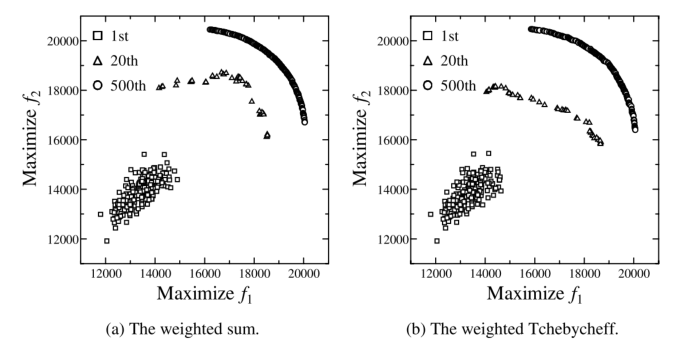
\includegraphics{cellular_moead_files/figure-beamer/unnamed-chunk-1-1.pdf}

\tiny From \citet{ishibuchi2009adaptation}.

\end{frame}

\subsection{Pareto Set}\label{pareto-set-1}

\begin{frame}{Non-dominated solutions}

\begin{enumerate}
\def\labelenumi{\arabic{enumi}.}
\tightlist
\item
  Let \(u = (u_1, ..., u_m)\) and \(v = (v_1, ..., v_m)\) vectors in
  \(\Omega\) (the decision space).

  \begin{itemize}
  \tightlist
  \item
    \(\forall i:u\) dominates \(v\) if \(f_i(u) \leq f_i(v)\) and
    \(\exists j:f_j(u) < f_j(v)\).
  \item
    u dominates v, v is dominated by u, u is better that v.
  \end{itemize}
\item
  A point \(x^*\) in \(\Omega\) is called \emph{Pareto Optimal} if no
  other point dominates \(x^*\). 
\end{enumerate}

\end{frame}

\subsection{Pareto Set}\label{pareto-set-2}

\begin{frame}{Pareto Front}

\centering
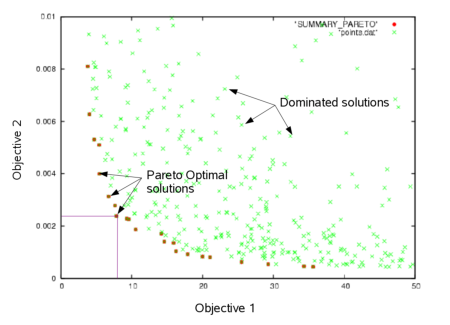
\includegraphics{cellular_moead_files/figure-beamer/unnamed-chunk-2-1.pdf}
\tiny From: \url{http://www.cenaero.be/Page.asp?docid=27103\&langue=EN}

\end{frame}

\begin{frame}{Pareto Front}

\begin{enumerate}
\def\labelenumi{\arabic{enumi}.}
\tightlist
\item
  The set of all Pareto Optimal is called the \emph{Pareto Set}.

  \begin{itemize}
  \tightlist
  \item
    \(P^*\) = \{\(x \in \Omega:\nexists y \in \Omega\) and
    \(F(y) \leq F(x)\)\}
  \end{itemize}
\item
  \textbf{Pareto Front} is the image of the Pareto Set in the objective
  space.

  \begin{itemize}
  \tightlist
  \item
    PF = \{\(F(x) = (f_i(x), ..., f_m(x)): x \in P^*\)\}
  \end{itemize}
\end{enumerate}

\end{frame}

\section{MOEA/D}\label{moead}

\subsection{MOEA/D}\label{moead-1}

\begin{frame}{Decompostion}

MOEA/D represents a class of population-based meta-heuristics for
solving Multi Objective Problems (MOPs).

\begin{itemize}
\tightlist
\item
  It is based on decomposition - one kind of scalarizing function
\item
  One multi-objective problem becomes various single-objective
  sub-problems. 
\item
  A decomposition strategy generates weight vectors that defines the
  sub-problems.
\end{itemize}

\end{frame}

\begin{frame}{Decomposition - 2 and 3 objective functions}

\centering
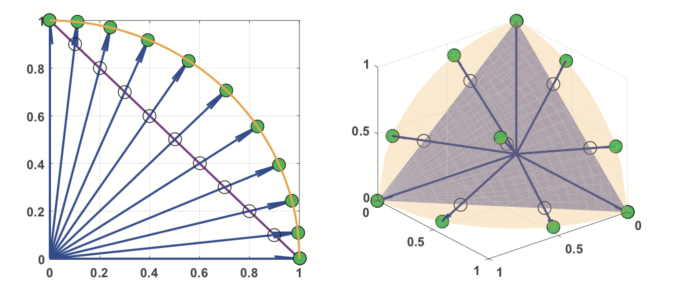
\includegraphics{cellular_moead_files/figure-beamer/unnamed-chunk-3-1.pdf}

\tiny From: \citet{chugh2017handling}.

\end{frame}

\subsection{MOEA/D}\label{moead-2}

\begin{frame}{Why use decomposition?}

\begin{itemize}
\tightlist
\item
  It may be good at generating an even distribution of solutions in
  MOPs;
\item
  It reduces the computation complexity when compared to other
  algorithms (NSGA-II) (at each generation),
  \citet{zhang2009performance}; 
\item
  Fitness assignment and diversity maintenance become easier to handle.
\end{itemize}

\end{frame}

\begin{frame}{Decomposition + Aggregation Function}

\centering
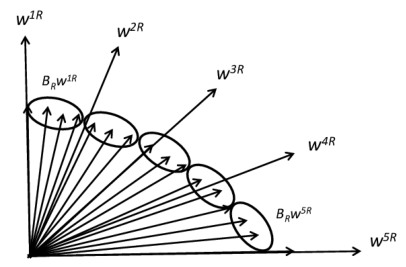
\includegraphics{cellular_moead_files/figure-beamer/unnamed-chunk-4-1.pdf}
\raggedright \tiny  \centering
\(f_{3}(x) = F * w_{3}\)

In general, \(f_{i}(x) = F * w_{i}\) Figure from:
\citet{chugh2017handling}.

\end{frame}

\subsection{MOEA/D}\label{moead-3}

\begin{frame}{Components of the MOEA/D}

\begin{itemize}
\tightlist
\item
  Decomposition strategy: decomposes w/ weight vectors;
\item
  Aggregation function: weight vector =\textgreater{} single-objective
  sub-problems;
\item
  Neighbourhood assignment strategy: Relationship between sub-problems;
\item
  Variation Stack: New candidates solutions;
\item
  Update Strategy: Maintain/discard candidate solutions;
\item
  Constraint handling method: Constraint violation;
\item
  Termination Criteria: when to stop the search.
\end{itemize}

\end{frame}

\section{Modifications - MOEA/D}\label{modifications---moead}

\subsection{Modifications}\label{modifications}

\begin{frame}{Modifications Already Integrated}

\begin{enumerate}
\def\labelenumi{\arabic{enumi}.}
\tightlist
\item
  Cellular GA - proposed in the context of MOEA/D by
  \citet{ishibuchi2009adaptation}.
\item
  Latin Hypercube Sample - an alternative approach in initializing
  populations.
\item
  On-line Resource Allocation - proposed in the context of MOEA/D by
  \citet{zhou2016all}.
\item
  Bet-and-Run: A kind of restart strategy - in the context of
  single-objective problems (SOP) by \citet{friedrich2017generic}
\end{enumerate}

\end{frame}

\subsection{Cellular GA}\label{cellular-ga}

\begin{frame}{Cellular GA and MOEA/D \citet{ishibuchi2009adaptation}}

\begin{itemize}
\tightlist
\item
  Why? MOEA/D can be viewed as a Cellular GA (cGA).

  \begin{itemize}
  \tightlist
  \item
    A cell can be seen as a specific ``Neighbourhood assignment
    strategy'', where each cell has its own weight vector.
  \end{itemize}
\item
  cGA is well explored in the context of SOP.
\end{itemize}

\end{frame}

\begin{frame}{MOEA/D as cGA}

\begin{itemize}
\tightlist
\item
  The main characteristic feature of MOEA/D as a cGA is the use of
  \textbf{local replacement} in addition to local selection.

  \begin{itemize}
  \tightlist
  \item
    Generated offspring for a cell is compared with not only the current
    solution of the cell but also its neighbours for possible
    replacement.
  \end{itemize}
\item
  Local replacement neighbourhood has greater effect on the performance
  than local selection neighbourhood.

  \begin{itemize}
  \tightlist
  \item
    Increasing its size tends to be better.
  \end{itemize}
\end{itemize}

\end{frame}

\subsection{Latin Hypercube Sample}\label{latin-hypercube-sample}

\begin{frame}{What is Latin Hypercube Sample}

\begin{itemize}
\tightlist
\item
  Latin Hypercube Sample (LHS) was developed to generate a distribution
  of collections of parameter values from a multidimensional
  distribution, for more information see \citet{stein1987large}.
\end{itemize}

\end{frame}

\begin{frame}{How it affects MOEA/D}

\begin{itemize}
\item
  As defined in \citet{mckay1979comparison}, it could be a good method
  to use for selecting values of input variables.
\item
  Therefore we expect that by using it, the initial population (ours
  input variable) would be better distributed along the search space.
\end{itemize}

\end{frame}

\subsection{\texorpdfstring{Online Resource Allocation -
\citet{zhou2016all}.}{Online Resource Allocation - @zhou2016all.}}\label{online-resource-allocation---zhou2016all.}

\begin{frame}{What is Online Resource Allocation}

\begin{itemize}
\tightlist
\item
  On-line Resource Allocation (ONRA) is an adaptation strategy that aim
  to adjust the behaviour of an algorithm in an on-line manner to suit
  the problem in question.
\end{itemize}

\end{frame}

\begin{frame}{How it affects MOEA/D - \citet{zhou2016all}.}

\begin{itemize}
\item
  Some sub-problems can be more difficult to approximate that others. To
  better explore them, different computational resources are allocated
  to different sub-problems.
\item
  The resources re-allocated is \emph{the number of functions
  evaluations}.

  \begin{itemize}
  \tightlist
  \item
    From an equal amount to every sub-problem to an amount related to
    the difficulty of the sub-problem.
  \end{itemize}
\end{itemize}

\end{frame}

\subsection{Restart Strategy}\label{restart-strategy}

\begin{frame}{What is Restart Strategy}

\begin{itemize}
\item
  Restart Strategy is a strategy used to avoid heavy-tailed running time
  distributions \citet{gomes2000heavy}.
\item
  If a execution of an algorithm does not conclude within a
  pre-determined limit or if the solution quality is unsatisfactory, we
  restart the algorithm \citet{lissovoi2017theoretical}.
\end{itemize}

\end{frame}

\begin{frame}{Bet-and-Run framework}

\begin{itemize}
\item
  It is defined in \citet{fischetti2014exploiting}. as a number of short
  runs with randomized initial conditions, bet on the most promising
  run, and bring it to completion.
\item
  To the best of our knowledge, only applied with EA in the context of
  SOP.
\end{itemize}

\end{frame}

\begin{frame}{How it affects MOEA/D - \citet{lissovoi2017theoretical}.}

\begin{itemize}
\item
  Initialisation can have a small beneficial effect even on very easy
  functions.
\item
  Countermeasure when problems with promising and deceptive regions are
  encountered.
\item
  Additional speed-up heuristic.
\end{itemize}

\end{frame}

\section{Evaluation Metrics}\label{evaluation-metrics}

\subsection{Indicators}\label{indicators}

\begin{frame}{Unary Indicators}

\begin{itemize}
\tightlist
\item
  Measure Pareto Sets independently.
\item
  Power is restricted.

  \begin{itemize}
  \tightlist
  \item
    Cannot tell in general if a set is better than another.
  \end{itemize}
\item
  Focus on problem dependent and specifics.

  \begin{itemize}
  \tightlist
  \item
    Assumptions and knowledge should be specified.
  \end{itemize}
\end{itemize}

\begin{enumerate}
\def\labelenumi{\arabic{enumi}.}
\tightlist
\item
  Hyper-volume.
\item
  Error ratio.
\item
  Distance from reference set.
\end{enumerate}

\end{frame}

\begin{frame}{Binary Indicators}

\begin{itemize}
\tightlist
\item
  Theoretically have no limitations.
\item
  Analysis and presentation of results more difficult.
\end{itemize}

\begin{enumerate}
\def\labelenumi{\arabic{enumi}.}
\tightlist
\item
  R1, R2, R3 indicators.
\item
  \(\varepsilon\)-Indicator.
\item
  Binary Hyper-volume.
\end{enumerate}

\end{frame}

\subsection{Hypervolume}\label{hypervolume}

\begin{frame}{Considerations}

\begin{itemize}
\tightlist
\item
  Is complete - If, and only if \(HV(A) > HV(B) \implies A\) is not
  worse than \(B\).
\item
  Is weakly compatible - \(HV(A) > HV(B) \implies\not B\) dominates
  \(A\).
\item
  Assumptions - All points of a Pareto Set under consideration dominate
  the reference point.

  \begin{itemize}
  \tightlist
  \item
    Ishibuchi \citet{ishibuchi2018specify} proposed a method to specify
    the reference point from a viewpoint of fair performance comparison.
  \end{itemize}
\end{itemize}

\end{frame}

\begin{frame}{Considerations}

\begin{itemize}
\tightlist
\item
  A large population size is \textbf{always} more beneficial than a
  small one.
\item
  Measures both the convergence toward the Pareto Front and the
  diversity of non-dominated solutions.
\item
  A monotonic increase of the hyper-volume over time cannot always be
  ensured.

  \begin{itemize}
  \tightlist
  \item
    For MOEA/D that is always true.
  \end{itemize}
\end{itemize}

\end{frame}

\subsection{\texorpdfstring{\(\varepsilon\)-Indicator}{\textbackslash{}varepsilon-Indicator}}\label{varepsilon-indicator}

\begin{frame}{Considerations}

\begin{itemize}
\tightlist
\item
  It compares 2 Pareto Sets.

  \begin{itemize}
  \tightlist
  \item
    It indicates which set is better and how much better
  \end{itemize}
\item
  If A is better than B \(\implies I_{\varepsilon}(B,A) > 0\).
\item
  If \(I_{\varepsilon}(A,B) \leq 0\) and
  \(I_{\varepsilon}(B,A) > 0 \implies A\) is better than \(B\).
\end{itemize}

\end{frame}

\section{Pilot Experiments}\label{pilot-experiments}

\subsection{Preliminary Results}\label{preliminary-results}

\begin{frame}{Experimental Design}

\begin{enumerate}
\def\labelenumi{\arabic{enumi}.}
\tightlist
\item
  Simple experiments - Check my understand and get insights.
\item
  DTLZ1, DTLZ2, DTLZ6 and DTLZ7 MOP benchmark functions - Available from
  the MOEADr package.
\item
  Every variation will be discussed based on the pilot data showed in
  the next slide by a box-plot figure.
\item
  Number of evaluations: 5 * 10 \^{} 4.
\item
  Based on the common variation: MOEA/D (variations 1 and 2 from MOEADr)
  and MOEA/D-DE.
\end{enumerate}

\end{frame}

\begin{frame}{Boxplot - HV}

\centering
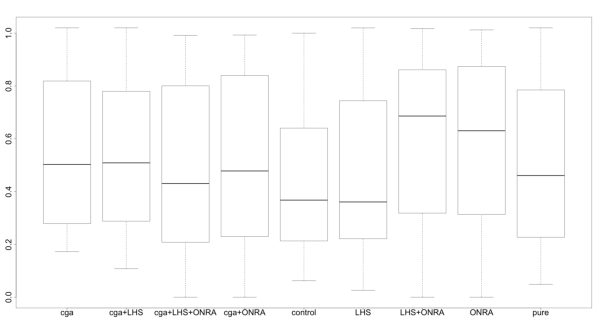
\includegraphics{cellular_moead_files/figure-beamer/unnamed-chunk-5-1.pdf}

\end{frame}

\subsection{Discussions}\label{discussions}

\begin{frame}{cGA}

\begin{enumerate}
\def\labelenumi{\arabic{enumi}.}
\tightlist
\item
  MOEA/D as cGA has a high sensitivity on the parameters of local
  replacement and local selection.
\item
  Decreasing the size of competition neighbourhood increases. the
  non-dominated solutions, but degrades the search ability of the
  MOEA/D. \textbf{As already observed in \citet{ishibuchi2009adaptation}
  }.
\end{enumerate}

\end{frame}

\begin{frame}{LHS}

\begin{enumerate}
\def\labelenumi{\arabic{enumi}.}
\tightlist
\item
  In some cases improves the results by a little.
\item
  It is cheap in terms of computational cost - it is only used once at
  each execution.
\end{enumerate}

\begin{itemize}
\tightlist
\item
  This improve seems not to be significant.
\end{itemize}

\end{frame}

\begin{frame}{ONRA}

\begin{enumerate}
\def\labelenumi{\arabic{enumi}.}
\tightlist
\item
  Computational costly -\textgreater{} more interactions than without it
  and we need to calculate the resources allocation every interaction.
\item
  It was beneficial in a few cases, while in others the overall quality
  decreased.

  \begin{itemize}
  \tightlist
  \item
    Considering the all functions and algorithms together it seems it
    leads to better results.
  \end{itemize}
\end{enumerate}

\end{frame}

\begin{frame}{Bet-and-Run Strategy}

\begin{enumerate}
\def\labelenumi{\arabic{enumi}.}
\tightlist
\item
  Overall, this strategy combined with the MOEA/D lead to better final
  quality results.
\item
  Its performances become better when combined with other variations,
  specially with cGA+LHS.
\end{enumerate}

\end{frame}

\begin{frame}{Future works}

\begin{enumerate}
\def\labelenumi{\arabic{enumi}.}
\tightlist
\item
  cGA - On the fly parameter adaptation.
\item
  ONRA

  \begin{itemize}
  \tightlist
  \item
    Review my implementation and try the other methods proposed in
    \citet{zhou2016all}. Only the one considered to be the ``best'' was
    implemented.
  \end{itemize}
\item
  Bet-and-Run strategy
\end{enumerate}

\begin{itemize}
\tightlist
\item
  Use this strategy to add some adaptive technique.
\item
  Use more instances based on the best one, instead of only one.
\item
  Dynamic bet-and-run.
\item
  Hierarchical bet-and-run - here it has only 2 phases.
\end{itemize}

\end{frame}

\subsection{References}\label{references}

\small

\begin{frame}[allowframebreaks]{}
\bibliographytrue
\bibliography{bib.bib}
\end{frame}

\section[]{}
\frame{\tiny \frametitle{Table of Contents}
\tableofcontents}

\end{document}
